% ChatGPT Directions 0 :  
% This is a Tbox Problem set for the following standards: 6.NS.C.6, 6.NS.C.7 
%--------------------------------------------------
\documentclass[12pt]{article}
\usepackage[a4paper, top=0.8in, bottom=0.7in, left=0.8in, right=0.8in]{geometry}
\usepackage{amsmath}
\usepackage{amsfonts}
\usepackage{latexsym}
\usepackage{graphicx}
\usepackage{fancyhdr}
\usepackage{tcolorbox}
\usepackage{enumitem}
\usepackage{setspace}
\usepackage{pgfplots}
\usepackage[defaultfam,tabular,lining]{montserrat} % Font settings for Montserrat

% General Comment: Template for creating problem sets in a structured format with headers, titles, and sections.
% This document uses Montserrat font and consistent styles for exercises, problems, and performance tasks.

% -------------------------------------------------------------------

%    - Include a header with standards and topic title: \fancyhead[L]{\textbf{<Standards>: <Topic Title>}}.
%    - Use "Problem Set:" as the prefix for subsection titles, followed by the topic title.
%    - Example: \subsection*{Problem Set: Understanding Number Lines and Inequalities}.
%
% 2. **Section Breakdown**:
%    - **Learning Objective**: A concise statement summarizing the goal of the problem set.
%    - **Exercises**: Focus on procedural fluency with straightforward tasks.
%    - **Problems**: Include moderately complex scenarios requiring reasoning or application.
%    - **Performance Task**: Real-world, open-ended tasks that require multi-step solutions or creative thinking.
%    - **Reflection**: Prompt students to reflect on their strategies and learning.
%
% -------------------------------------------------------------------

\setlength{\parindent}{0pt}
\pagestyle{fancy}

\setlength{\headheight}{27.11148pt}
\addtolength{\topmargin}{-15.11148pt}

\fancyhf{}
%\fancyhead[L]{\textbf{6.NS.C.6, 6.NS.C.7: Number Lines and Inequalities}} % Header with standards and topic title
\fancyhead[R]{\includegraphics[width=0.8cm]{Round Logo.png}} % Placeholder for logo
\fancyfoot[C]{\footnotesize © Study Smart Tutors}

\sloppy

\title{}
\date{}
\hyphenpenalty=10000
\exhyphenpenalty=10000

\pgfplotsset{compat=1.18}

\begin{document}

\subsection*{Problem Set: Number Lines and Inequalities}
\onehalfspacing

% Learning Objective Box
\begin{tcolorbox}[colframe=black!40, colback=gray!5, 
coltitle=black, colbacktitle=black!20, fonttitle=\bfseries\Large, 
title=Learning Objective, halign title=center, left=5pt, right=5pt, top=5pt, bottom=5pt]
\textbf{Objective:} \small Develop an understanding of how to locate numbers on a number line, compare rational numbers, and interpret inequalities in real-world contexts.
\end{tcolorbox}

% Exercises Box
\begin{tcolorbox}[colframe=black!60, colback=white, 
coltitle=black, colbacktitle=black!15, fonttitle=\bfseries\Large, 
title=Exercises, halign title=center, left=10pt, right=10pt, top=10pt, bottom=40pt]
\begin{enumerate}[itemsep=1.5em]
    \item Plot the following numbers on a number line: \( -3, 2.5, 0, -1.5, 4 \).
    \begin{center}
        \begin{tikzpicture}
            \draw[thick, <->] (-5.5,0) -- (5.5,0); % Number line
            \foreach \x in {-5,-4,-3,-2,-1,0,1,2,3,4,5} {
                \draw (\x,0.1) -- (\x,-0.1) node[below] {\x};
            }
        \end{tikzpicture}
    \end{center}
    
    \item Compare the numbers \( -7 \) and \( -4 \). Write the inequality and explain which is greater.
    
    \item Order the numbers \( 1.2, -0.8, 0, -1.5, 2.5 \) from least to greatest.
    
    \item Solve and graph: \( x + 3 \leq 5 \).
    \vspace{2em}
    \begin{center}
        \begin{tikzpicture}
            \draw[thick, <->] (-3,0) -- (6,0); % Number line
            \foreach \x in {-2,-1,0,1,2,3,4,5} {
                \draw (\x,0.1) -- (\x,-0.1) node[below] {\x};
            }
            
        \end{tikzpicture}
    \end{center}
    
    \item Write the inequality: "The temperature is less than or equal to \( -5^\circ \)C."
    
    \item Compare and write the inequality: \( 2.4 \) and \( 2.5 \).
    
   \item Plot and label \( -\frac{5}{6}, \frac{2}{3}, \frac{1}{2} \) on a number line.
\begin{center}
    \begin{tikzpicture}[scale=4.5] % Scaled up the number line for clarity
        % Draw the number line
        \draw[thick, <->] (-1.5,0) -- (1.5,0);
        
        % Tick marks
        \foreach \x in {-1,,-.33,-0.67,0,0.33, 0.67,1} {
            \draw (\x,0.1) -- (\x,-0.1) node[below] {\x};
        }
        
    \end{tikzpicture}
\end{center}

    \item Solve for \( y \): \( -4 \leq y + 2 < 3 \) and graph the solution. \vspace{2em}
    \begin{center}
        \begin{tikzpicture}
            \draw[thick, <->] (-5,0) -- (5,0); % Number line
            \foreach \x in {-4,-3,-2,-1,0,1,2,3} {
                \draw (\x,0.1) -- (\x,-0.1) node[below] {\x};
            }
            
        \end{tikzpicture}
    \end{center}
\end{enumerate}
\end{tcolorbox}

\vspace{1em}

% Problems Box
\begin{tcolorbox}[colframe=black!60, colback=white, 
coltitle=black, colbacktitle=black!15, fonttitle=\bfseries\Large, 
title=Problems, halign title=center, left=10pt, right=10pt, top=10pt, bottom=60pt]
\begin{enumerate}[start=9, itemsep=5em]
    % Problem 9
   \item A submarine is at \( -200 \) feet. It ascends \( 120 \) feet. Where is the submarine now on a number line? 

    \begin{tikzpicture}[scale=1.5]
        % Vertical number line
        \draw[thick, <->] (0,-2.5) -- (0,2); 
        
        % Tick marks and labels
        \foreach \y in {-2,-1,0,1} {
            \draw (-0.1,\y) -- (0.1,\y) node[right] {{\y00}};
        }
        
        
    \end{tikzpicture}


% Problem 10
\item The freezing point of a substance is \( -15^\circ \text{C} \), and its boiling point is \( 85^\circ \text{C} \). What is the range of temperatures where the substance is in a liquid state? Write an inequality to represent this.

 

   % Problem 11
\item A delivery truck’s load weight must be greater than \( 500 \) pounds and less than or equal to \( 1,000 \) pounds. 
\begin{enumerate}
    \item Write an inequality to represent the allowable range of the load weight.
    \item If the truck currently carries \( 620 \) pounds, is the load within the acceptable range? If so, how many more pounds can the truck carry?

\end{enumerate}


    % Problem 12
    \item Compare and explain: Which is greater, \( -2.7 \) or \( -2.9 \)? Write your answer as an inequality and explain.
 
        

\end{enumerate}
\end{tcolorbox}

\vspace{1em}

% Performance Task Box
\begin{tcolorbox}[colframe=black!60, colback=white, 
coltitle=black, colbacktitle=black!15, fonttitle=\bfseries\Large, 
title=Performance Task: Mountain Heights and Depths, halign title=center, left=10pt, right=10pt, top=10pt, bottom=110pt]
\textbf{Scenario:} A mountain peak is at \( 14,000 \) feet above sea level, and a nearby valley is \( -200 \) feet below sea level. A helicopter starts at the peak and descends to the valley.

\textbf{Task:}
\begin{enumerate}[itemsep=5em]
    \item Write the inequality representing the helicopter's altitude during the descent.
    \item Graph the altitude on a number line.
    \item If the helicopter stops halfway between the peak and the valley, what is its altitude? Show your work.
\end{enumerate}
\end{tcolorbox}

\vspace{1em}

% Reflection Box
\begin{tcolorbox}[colframe=black!60, colback=white, 
coltitle=black, colbacktitle=black!15, fonttitle=\bfseries\Large, 
title=Reflection, halign title=center, left=10pt, right=10pt, top=10pt, bottom=110pt]
What strategies did you use to locate numbers on a number line and solve inequalities?  Reflect on any challenges you encountered and how you overcame them.
\end{tcolorbox}

\end{document} 